\begin{figure}[htpb]
	\centering\capstart{}
	\subfloat[\(\Re\big\{\pixel{f_{A}}\big\}\)] % chktex 21
	{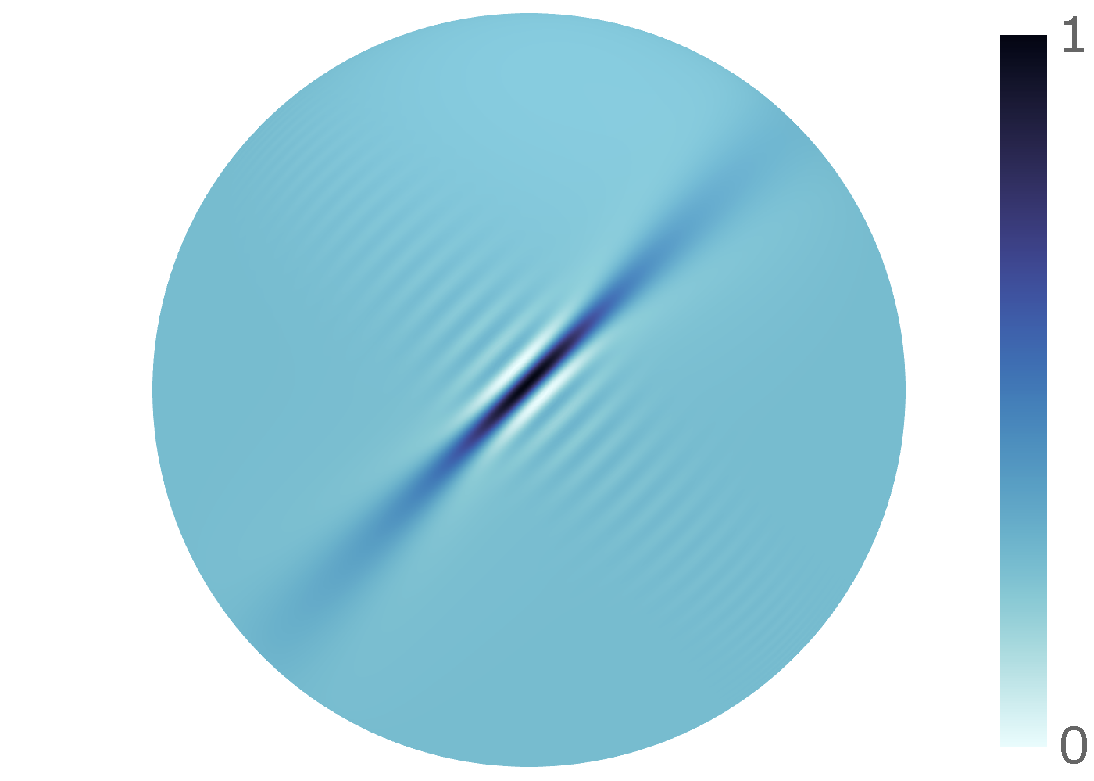
\includegraphics[trim={23 7 3 6},clip,width=.5\textwidth]{harmonic_gaussian_100lsig_10msig_L128_res512_real_norm.pdf}}
	\hfill
	\subfloat[\(\Re\big\{\pixel{f_{B}}\big\}\)]  % chktex 21
	{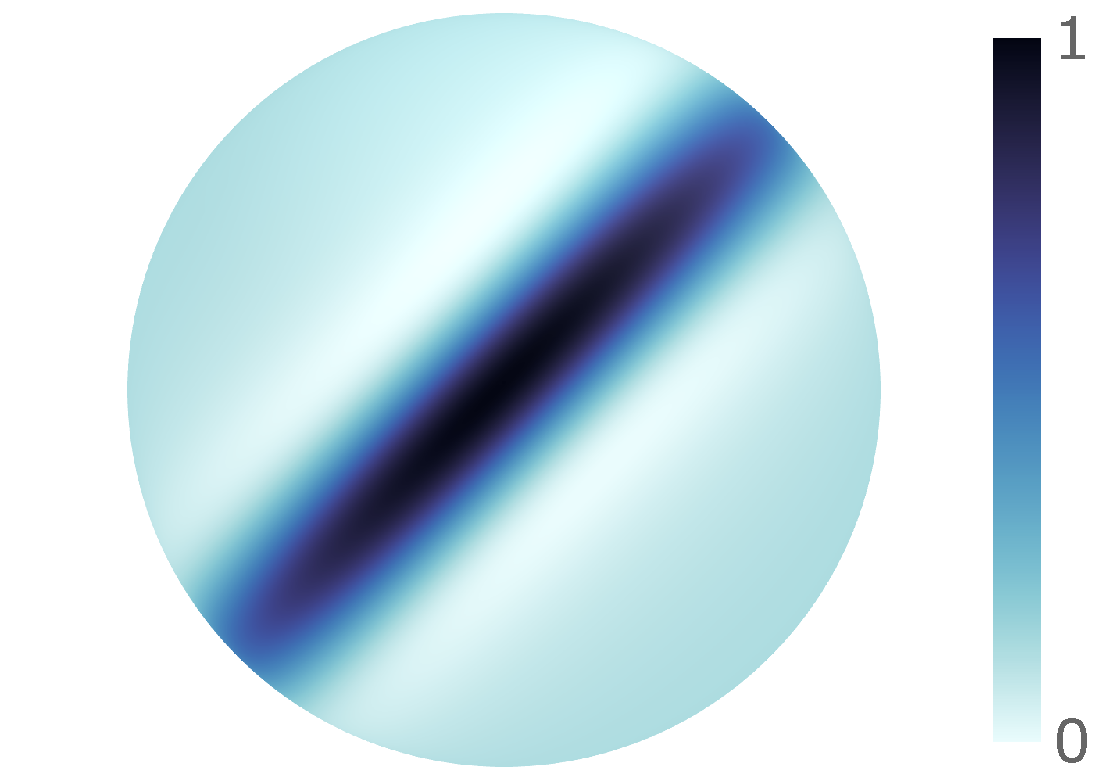
\includegraphics[trim={23 7 3 6},clip,width=.5\textwidth]{harmonic_gaussian_10lsig_10msig_L128_res512_real_norm.pdf}}
	\newline
	\subfloat[\(\Re\big\{\pixel{(\translation{\omega'}f_{A})}\big\}\)]  % chktex 21
	{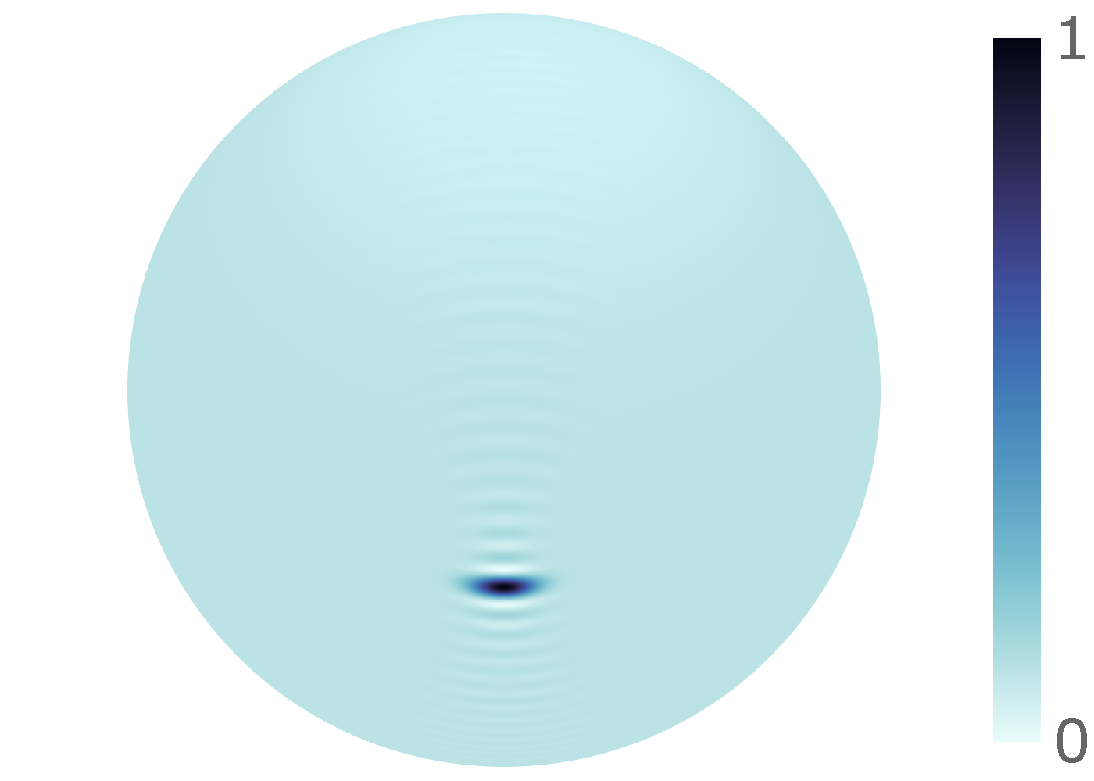
\includegraphics[trim={23 7 3 6},clip,width=.5\textwidth]{harmonic_gaussian_100lsig_10msig_L128_translate_alpha3pi4_beta1pi8_res512_real_norm.pdf}}
	\hfill
	\subfloat[\(\Re\big\{\pixel{(\translation{\omega'}f_{B})}\big\}\)]  % chktex 21
	{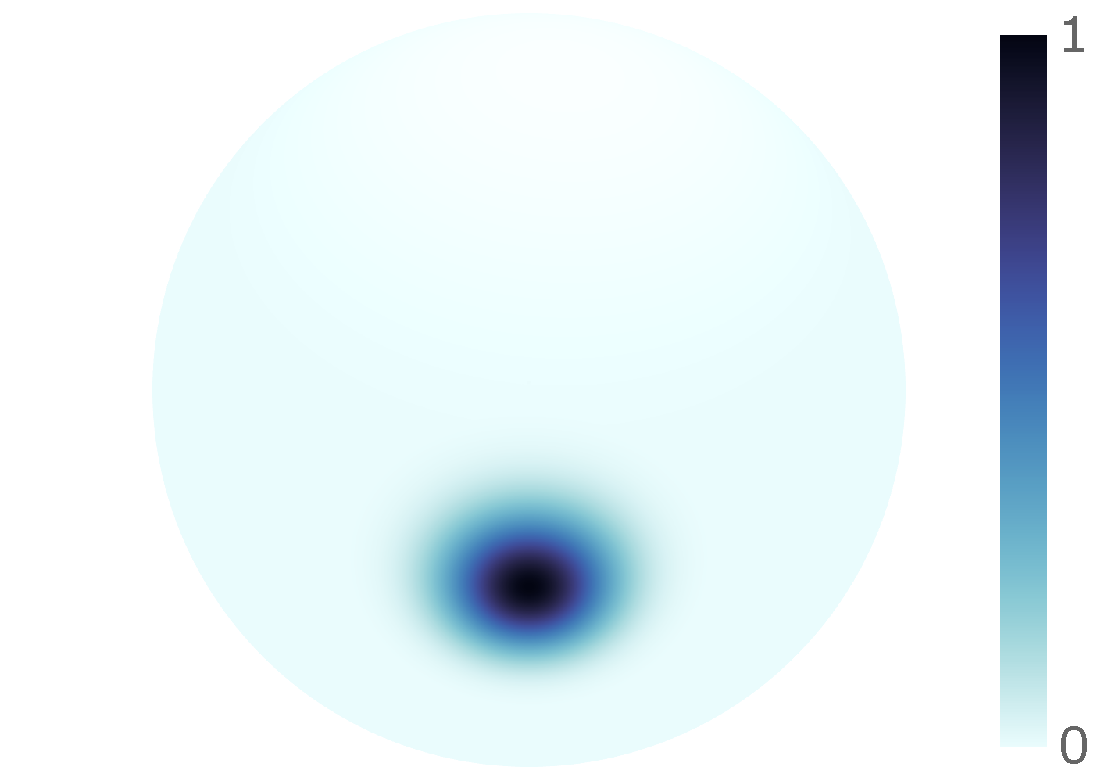
\includegraphics[trim={23 7 3 6},clip,width=.5\textwidth]{harmonic_gaussian_10lsig_10msig_L128_translate_alpha3pi4_beta1pi8_res512_real_norm.pdf}}
	\caption[
	Two harmonic Gaussians on the north pole and then translated
	]{
	The top row presents the harmonic Gaussian on the north pole (bandlimited at \(L=128\)) for two different \((\sigma_{\ell},\sigma_{m})\) values, \cf{} \cref{eq:chapter3_harmonic_gaussian}.
	Panel (a) corresponds to a more elongated kernel \(f_{A}\), where \((\sigma_{\ell},\sigma_{m}) = (10^{2},10^{1})\).
	The harmonic Gaussian is translated to some \(\omega'=(\theta',\phi')\) as shown in panel (c).
	Whereas panel (b) corresponds to a more symmetric kernel \(f_{B}\), where \((\sigma_{\ell},\sigma_{m}) = (10^{1},10^{1})\), with the corresponding translated function in panel (d).
	The colour is between zero and one, reflecting the scaled intensity of the field.
	}\label{fig:chapter3_harmonic_gaussian}
\end{figure}
